%%%%%%%%%%%%%%%%%%%%%%%%%%%%%%%%%%
\section{Results with collinear photon-PDFs}
%%%%%%%%%%%%%%%%%%%%%%%%%%%%%%%%%%

We start with the calculation of the elastic contribution, $p+\textrm{Pb}\rightarrow p+\textrm{Pb}+ \ell^+\ell^-$
for which the following parameterization is used~\cite{Budnev:1974de}:
\begin{equation} \label{eq:elasticRenat}
\gamma^{p}_{el}(x)  = \frac{\alpha_{\rm em}}{\pi}
\left(
\frac{1-x+0.5x^2}{x}
\right)
\left(
\frac{F+3}{F-1}\log{F}-\frac{17}{6}-\frac{4}{3F}+\frac{1}{6F^2}
\right)~,
\end{equation}
where $F = 1+\frac{Q_0^2(1-x)}{x^2 m_p^2}$ and $Q_0^2 = 0.71$~\GeV$^2$. This parameterization is a good analytical approximation of Eq.~\ref{proton_el_flux} integrated over $Q^2$.
The results for the elastic case are cross-checked with the calculation from STARlight MC and a good agreement between the fiducial cross-sections is found:
$\sigma_{fid}^{\textrm{el}} = 17.5$~nb, whereas $\sigma_{fid}^{\textrm{STARlight}} = 17.0$~nb.
Both calculations are also corrected by a factor $S^2=0.96$ which 
is calculated using STARlight, where the hard-sphere proton--nucleus requirement~\cite{Klein:2016yzr} is used.

Next, for the inelastic case ($\gamma p\rightarrow \ell^+\ell^- + X$), several recent parameterizations of the photon parton distributions are studied: CT14qed~\cite{Schmidt:2015zda}, HKR16qed~\cite{Harland-Lang:2016kog}, LUXqed17~\cite{Manohar:2017eqh} and NNPDF3.1luxQED~\cite{Bertone:2017bme}. 
All predictions are scaled by $S^2=0.95$, again derived from STARlight. This value of $S^2$ is lower than for the purely elastic case, due to slightly smaller average impact parameter between the proton and the ion in the inelastic reaction.
One should note that all of these PDF sets include both elastic and inelastic parts of the photon spectrum.
We keep the elastic part now (as provided by each group), but we subtract it later in Sec.~\ref{sec:discussion} for the comparison with $k_T$-factorization results.

The integrated fiducial cross-sections for $p+\textrm{Pb}\rightarrow \textrm{Pb} + \ell^+\ell^- + X$ production at $\sqrt{s_{N N}} = 8.16$~\TeV\ for different collinear photon PDF sets are summarized in Tab.~\ref{fig:xs}.
Comparison of several lepton kinematic distributions between different photon-PDFs is shown in Fig.~\ref{fig:inc_cut}, including invariant mass and rapidity of lepton pair, and single-lepton transverse momentum/pseudorapidity distributions. 
The asymmetry visible in pair rapidity and single-lepton pseudorapidity distributions is due to expermental setup, which assumes a difference in the energy per nucleon between the proton beam and the lead beam (see Sec.~\ref{sec:experiment}).
All photon PDF parameterizations agree within 20\% with each other.
The differences are mainly due to overall PDF normalization, as no variation in the shape of various kinematic distributions is observed.

To check the sensitivity to the nuclear form factor modelling (Eq.~\ref{pb_el_flux}), different values of $R_A$ ($R_A = 7.1$ fm) and $a$ ($a=0.55$ fm) parameters are used, in a similar way as in Ref.~\cite{Azevedo:2019fyz}. These variations change the fiducial cross-sections by 4\% and 3\% respectively.


\begin{table}[h!]
\begin{center}
\begin{tabular}{|l|c|c|}
\hline
Contribution & $p_T^{\ell} > 4$ \GeV & $p_T^{\ell}  > 4$ \GeV, $|\eta^{\ell}| < 2.4$,\\
& & $m_{\ell^+\ell^-} > 10$ \GeV\\
\hline
$\gamma^{p}_{\rm{el}}$  & 44.9 nb & 17.5 nb\\ % [Electric]
\hline
$\gamma^{p}_{\rm{el}} + \gamma^{p}_{\rm{inel}}$ [CT14qed\_inc] & $98\pm4$ (PDF) nb & $40\pm 2$ (PDF) nb\\
\hline
$\gamma^{p}_{\rm{el}} + \gamma^{p}_{\rm{inel}}$ [LUXqed17] & $105.8\pm0.2$ (PDF) nb & $44.1 \pm 0.1$ (PDF) nb\\
\hline
$\gamma^{p}_{\rm{el}} + \gamma^{p}_{\rm{inel}}$ [NNPDF3.1luxQED] & $115.6 \pm 0.6$ (PDF) nb & $45.9 \pm 0.3$ (PDF) nb\\
\hline
$\gamma^{p}_{\rm{el}} + \gamma^{p}_{\rm{inel}}$ [HKR16qed] & 121.6 nb & 49.4 nb\\
\hline
\end{tabular}
\end{center}
\caption{Integrated fiducial cross sections for $p+\textrm{Pb}\rightarrow \textrm{Pb} + \ell^+\ell^- + X$ production at $\sqrt{s_{N N}} = 8.16$~\TeV\ for different collinear photon PDF sets. 
The effect of applying only $p_T^{\ell}$ requirement is shown in second column.
The uncertainties denote the PDF uncertainties (if available) calculated at 68\% CL.
For comparison, the cross section for purely elastic contribution is also shown.}
\label{fig:xs}
\end{table}

\begin{figure}[]

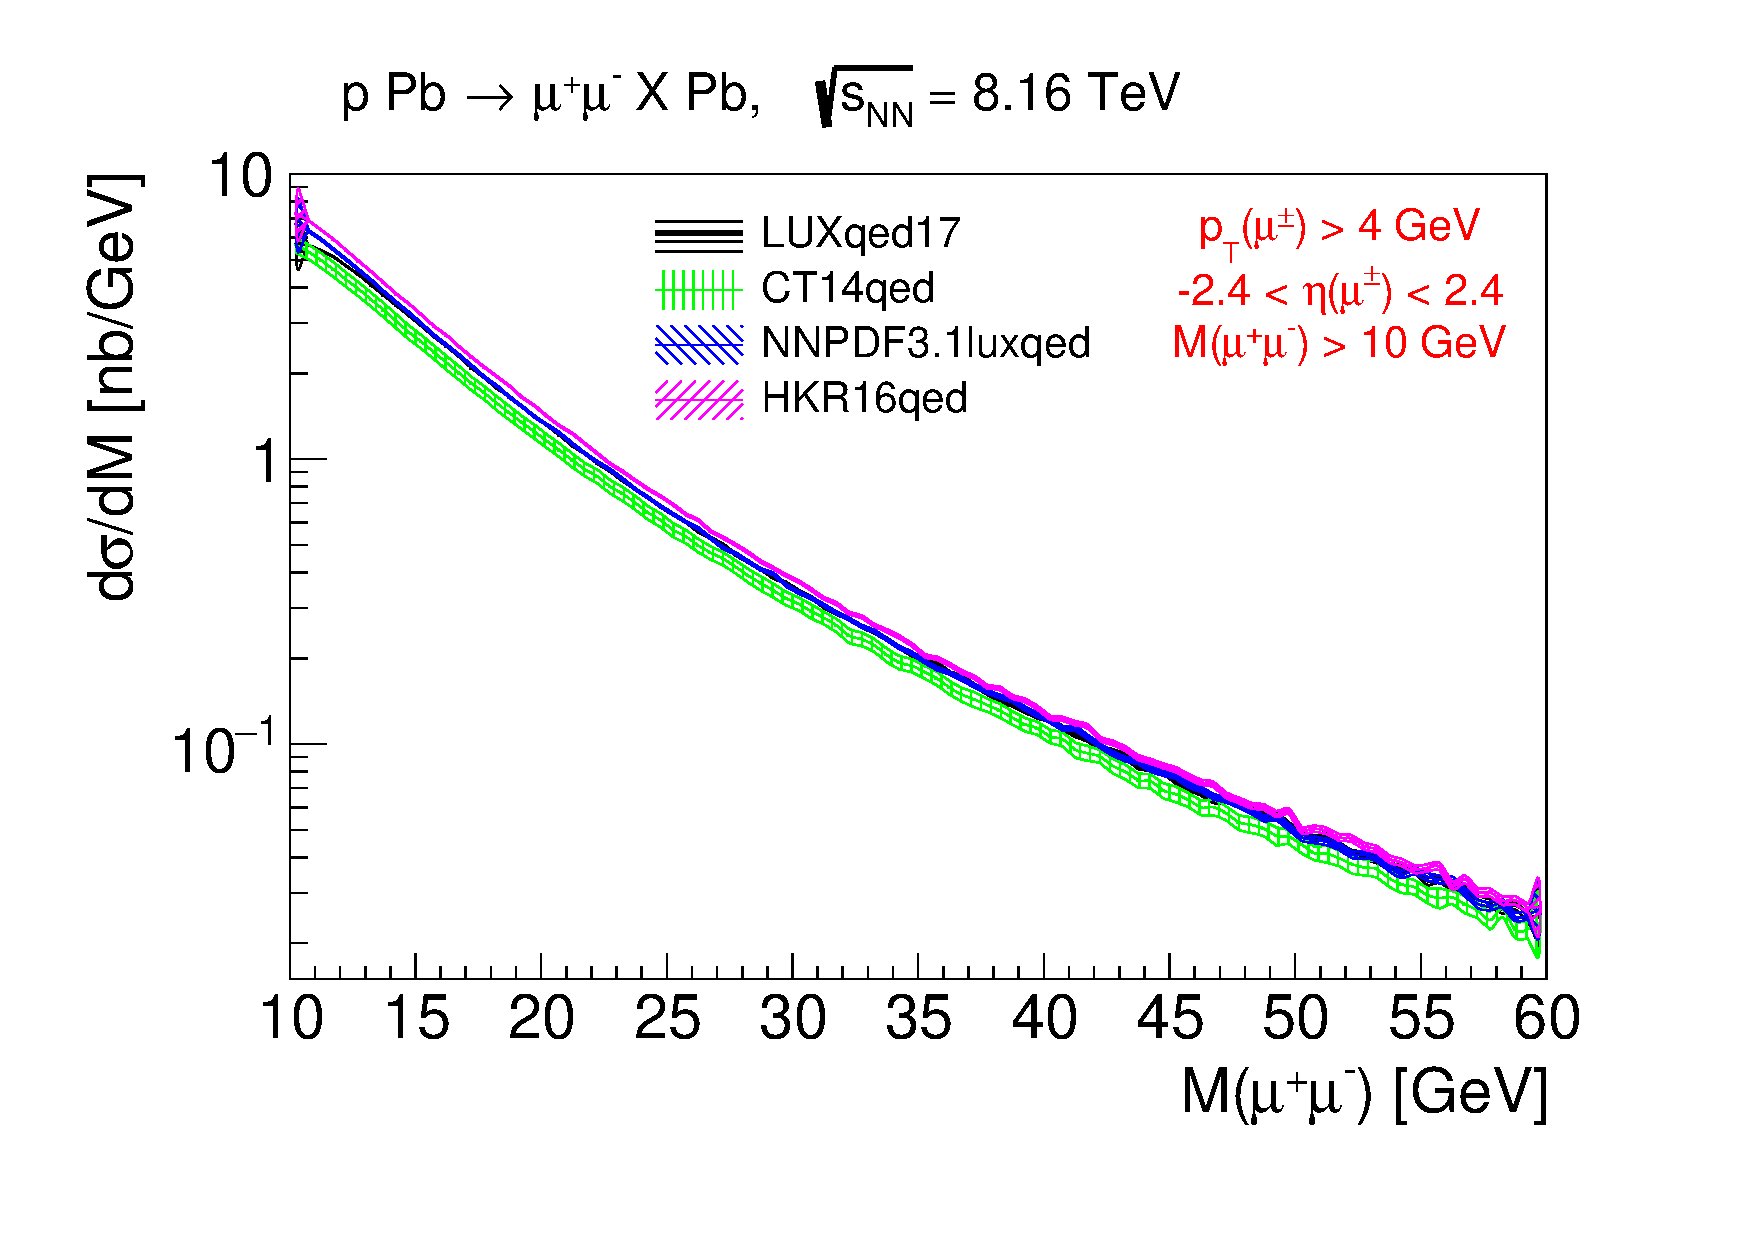
\includegraphics[width=0.43\textwidth]{figures/Mll_inc_cut.pdf}
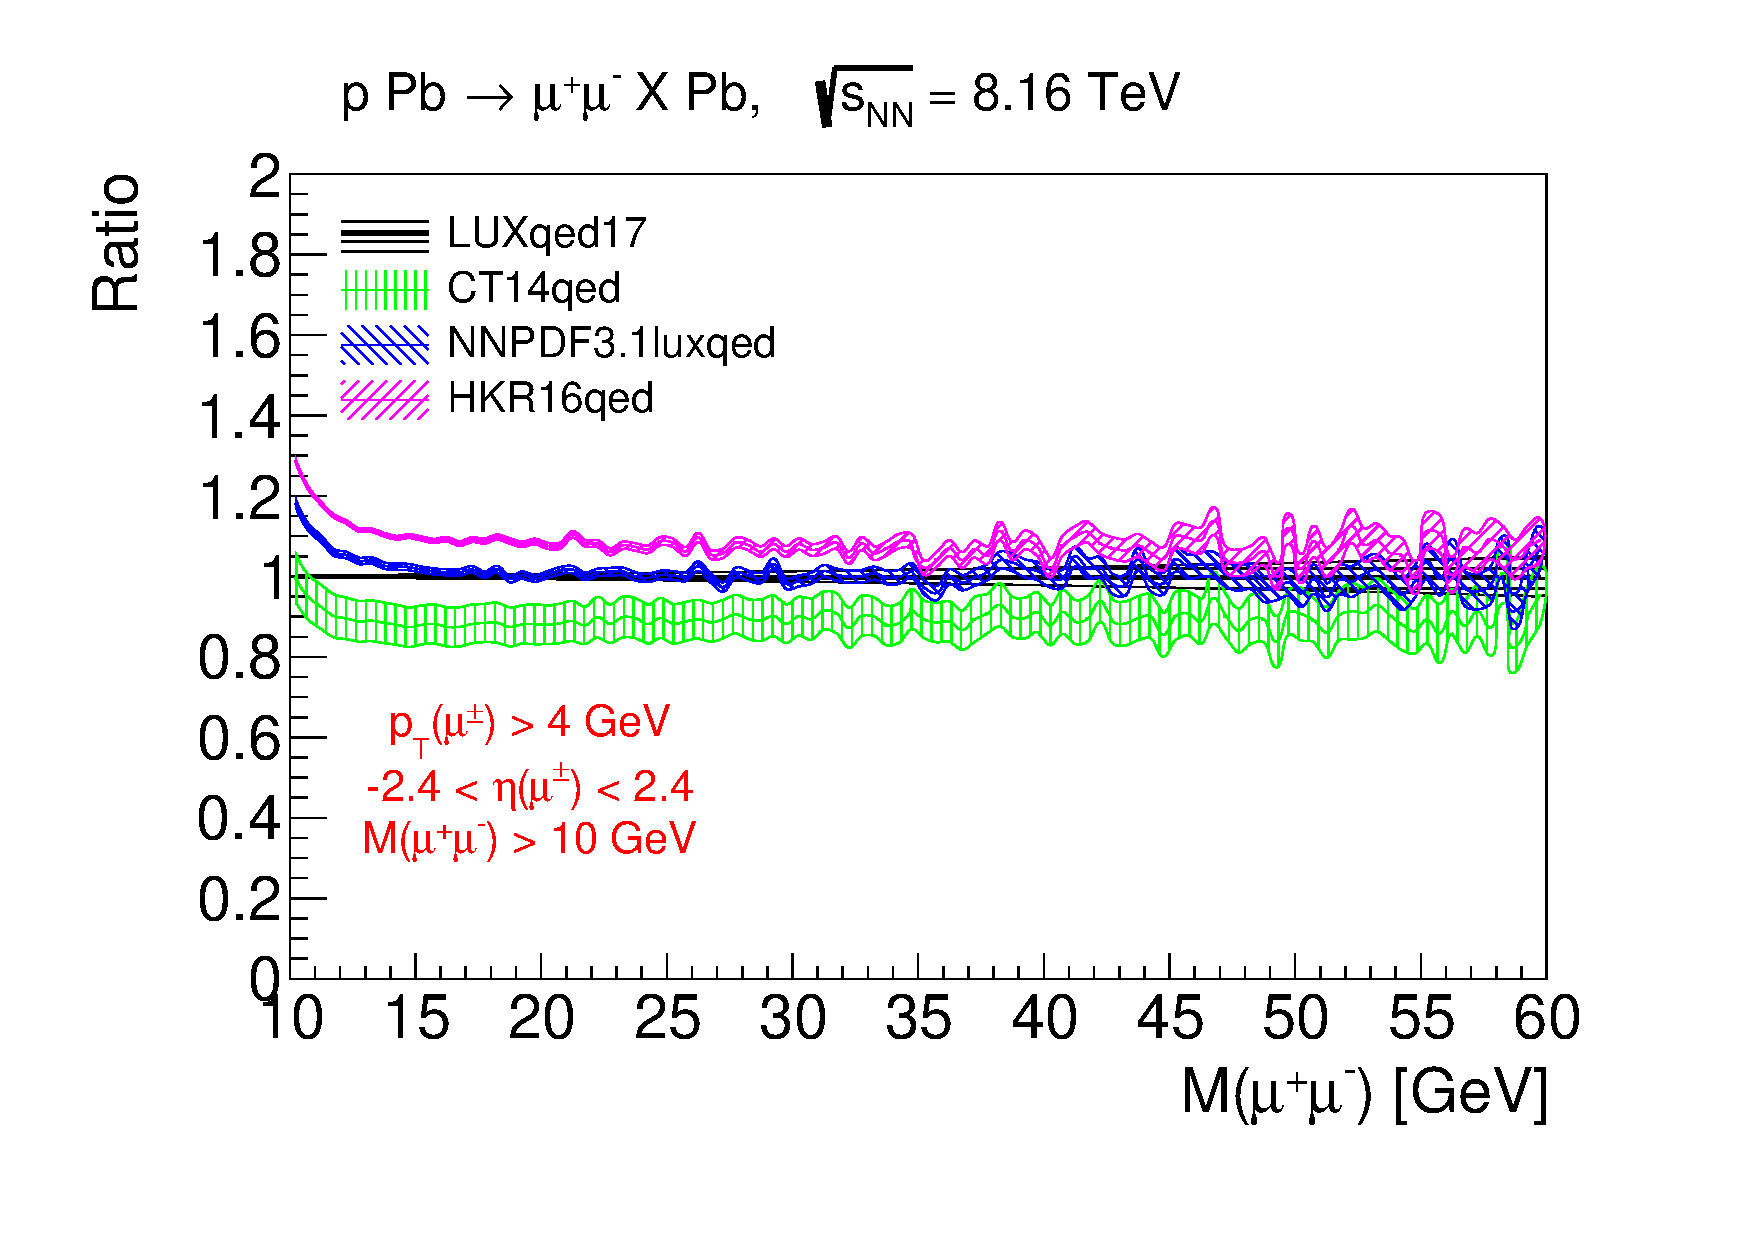
\includegraphics[width=0.43\textwidth]{figures/RatioMll_inc_cut.pdf}
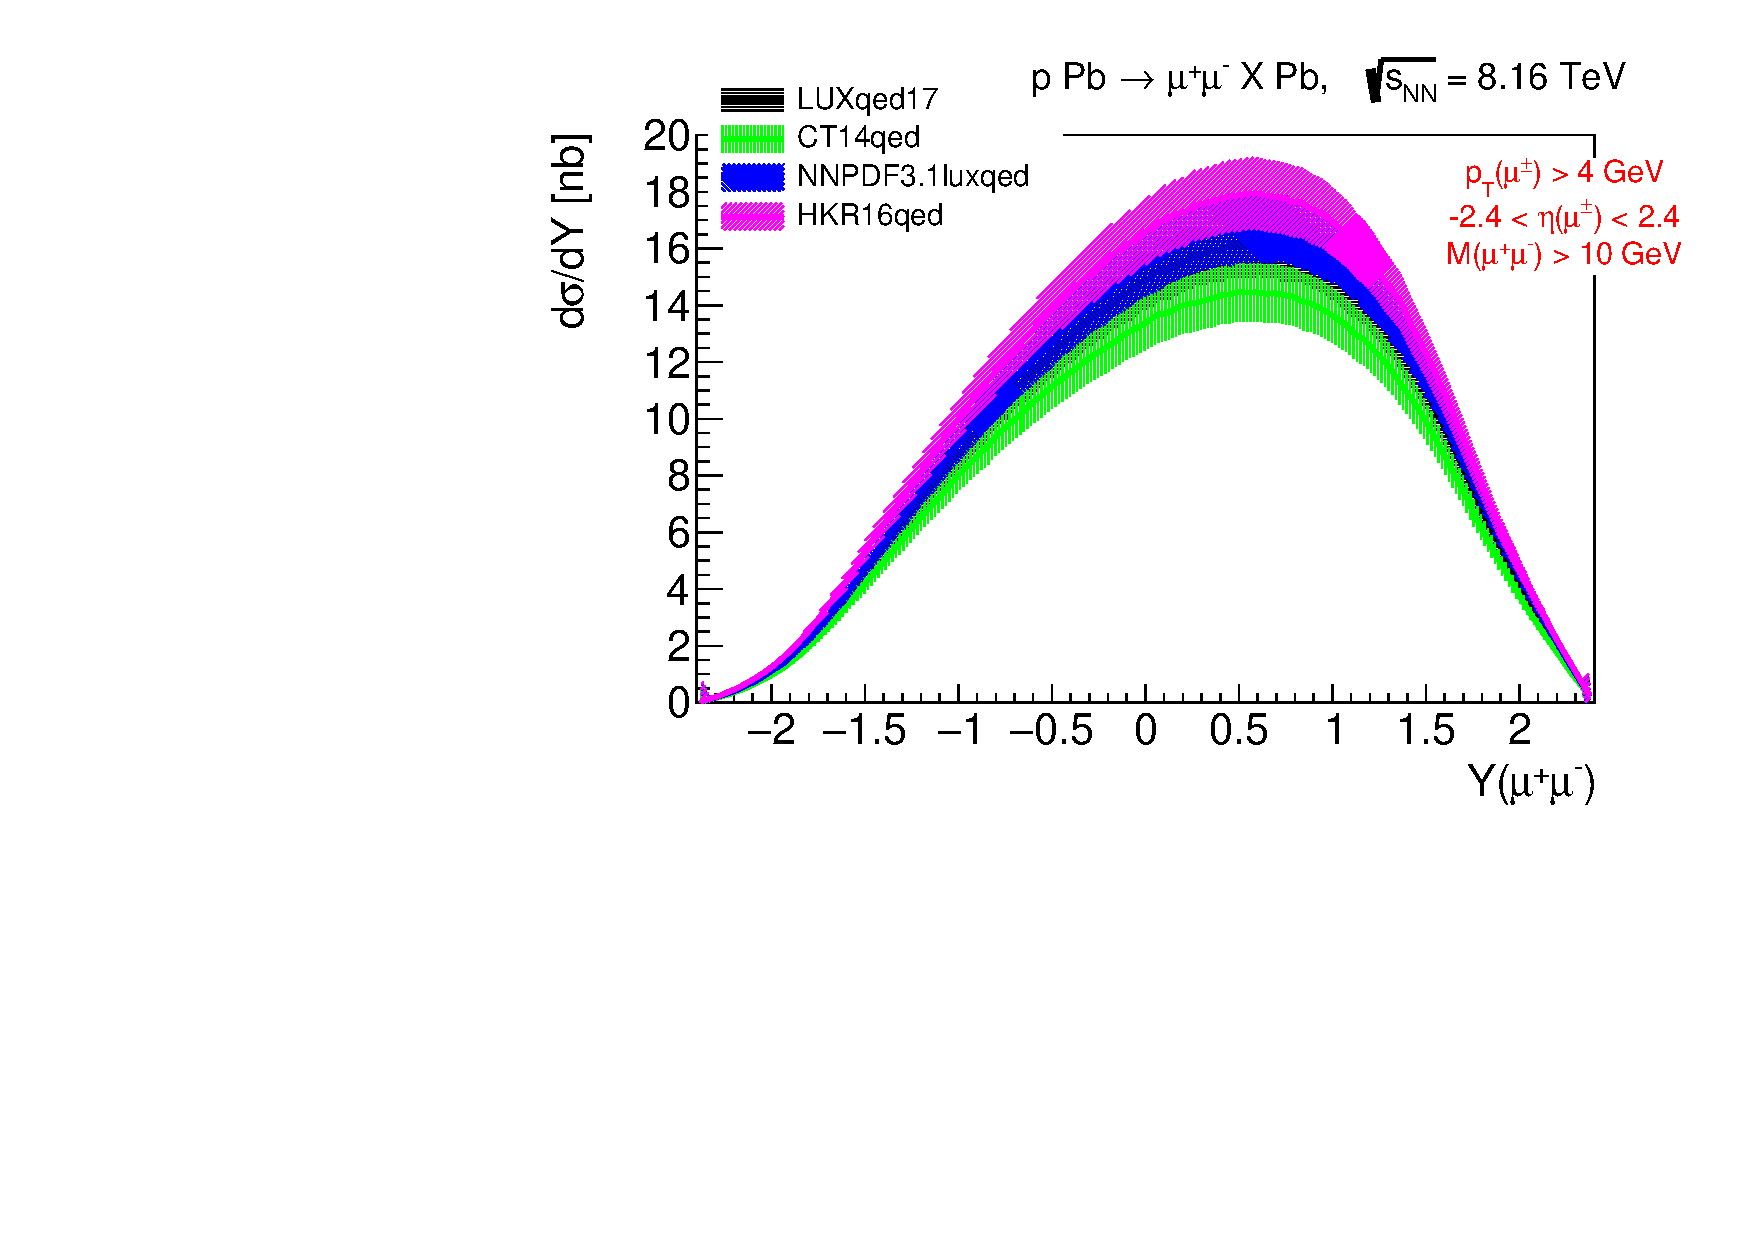
\includegraphics[width=0.43\textwidth]{figures/Yll_inc_cut.pdf}
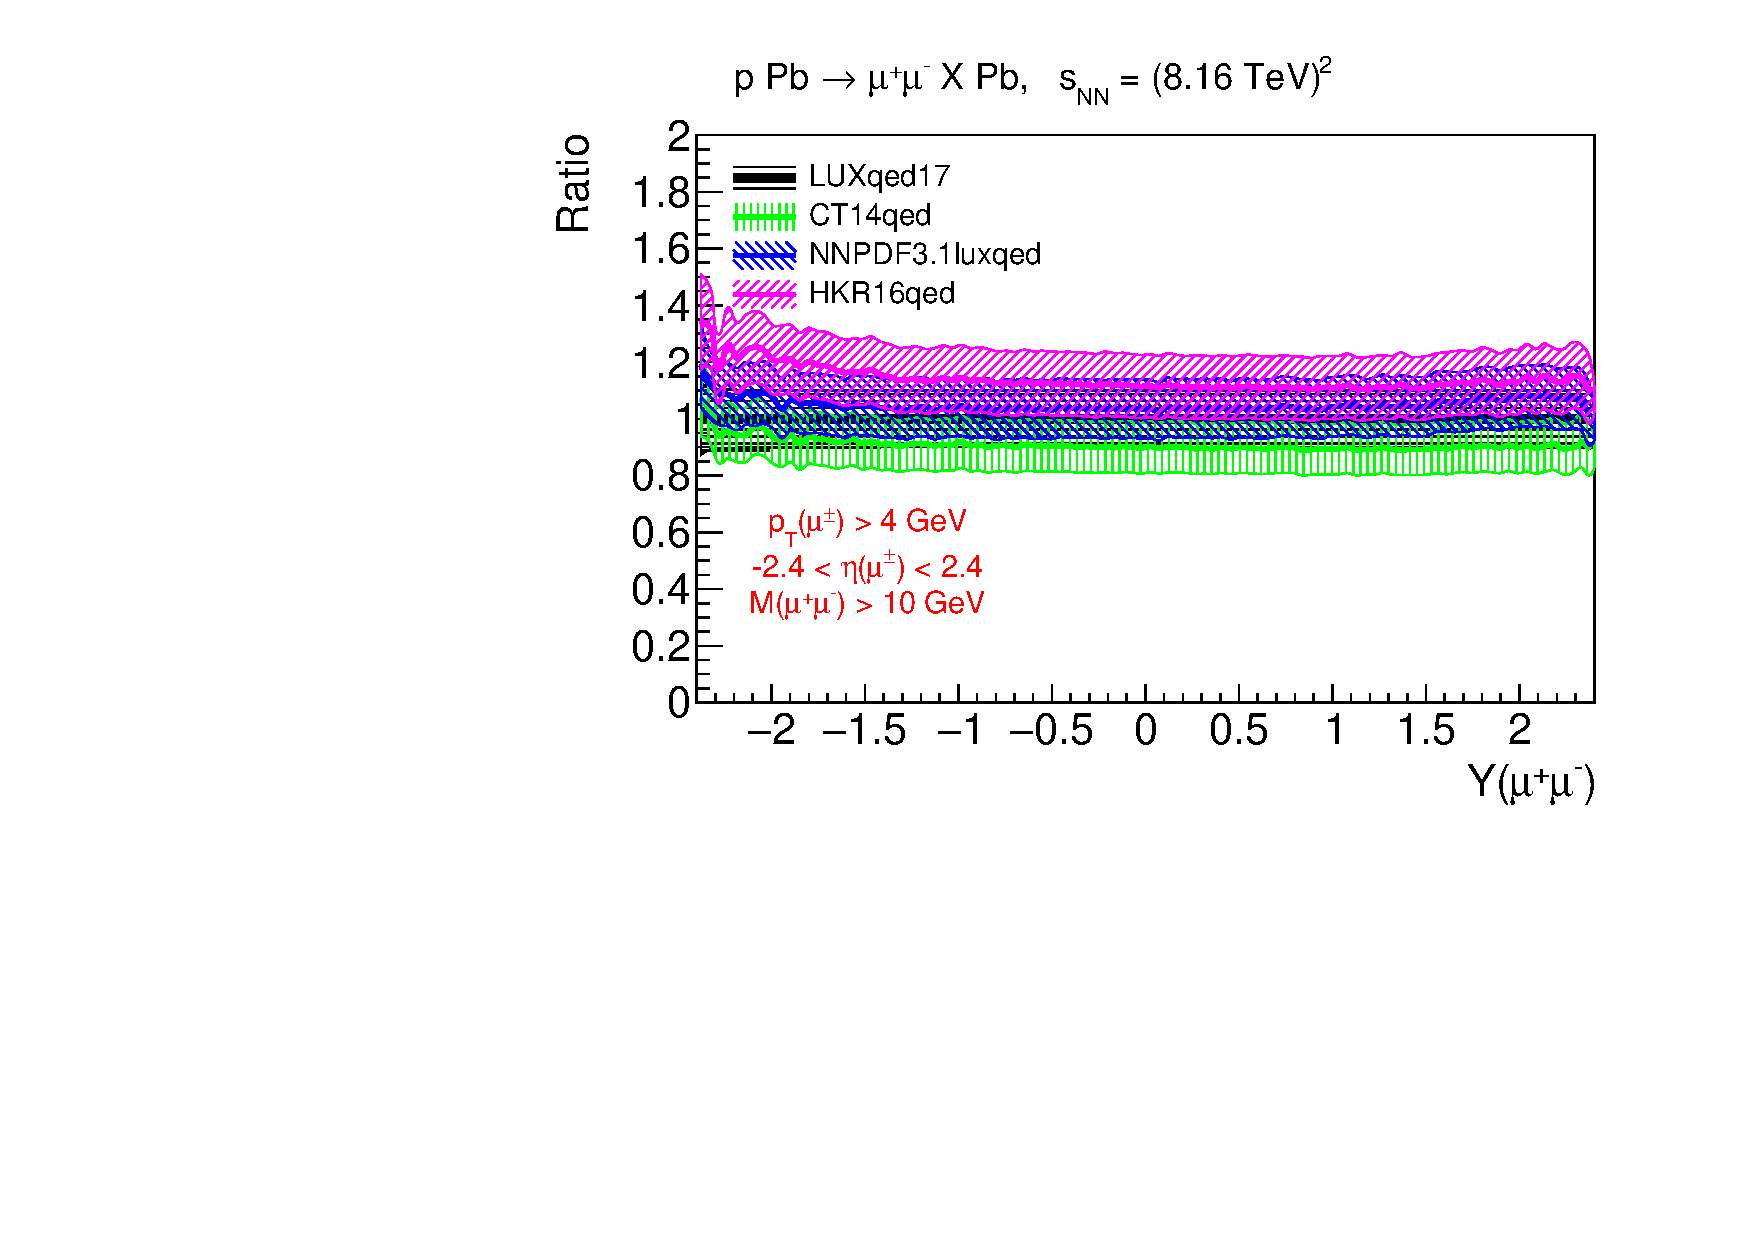
\includegraphics[width=0.43\textwidth]{figures/RatioYll_inc_cut.pdf}
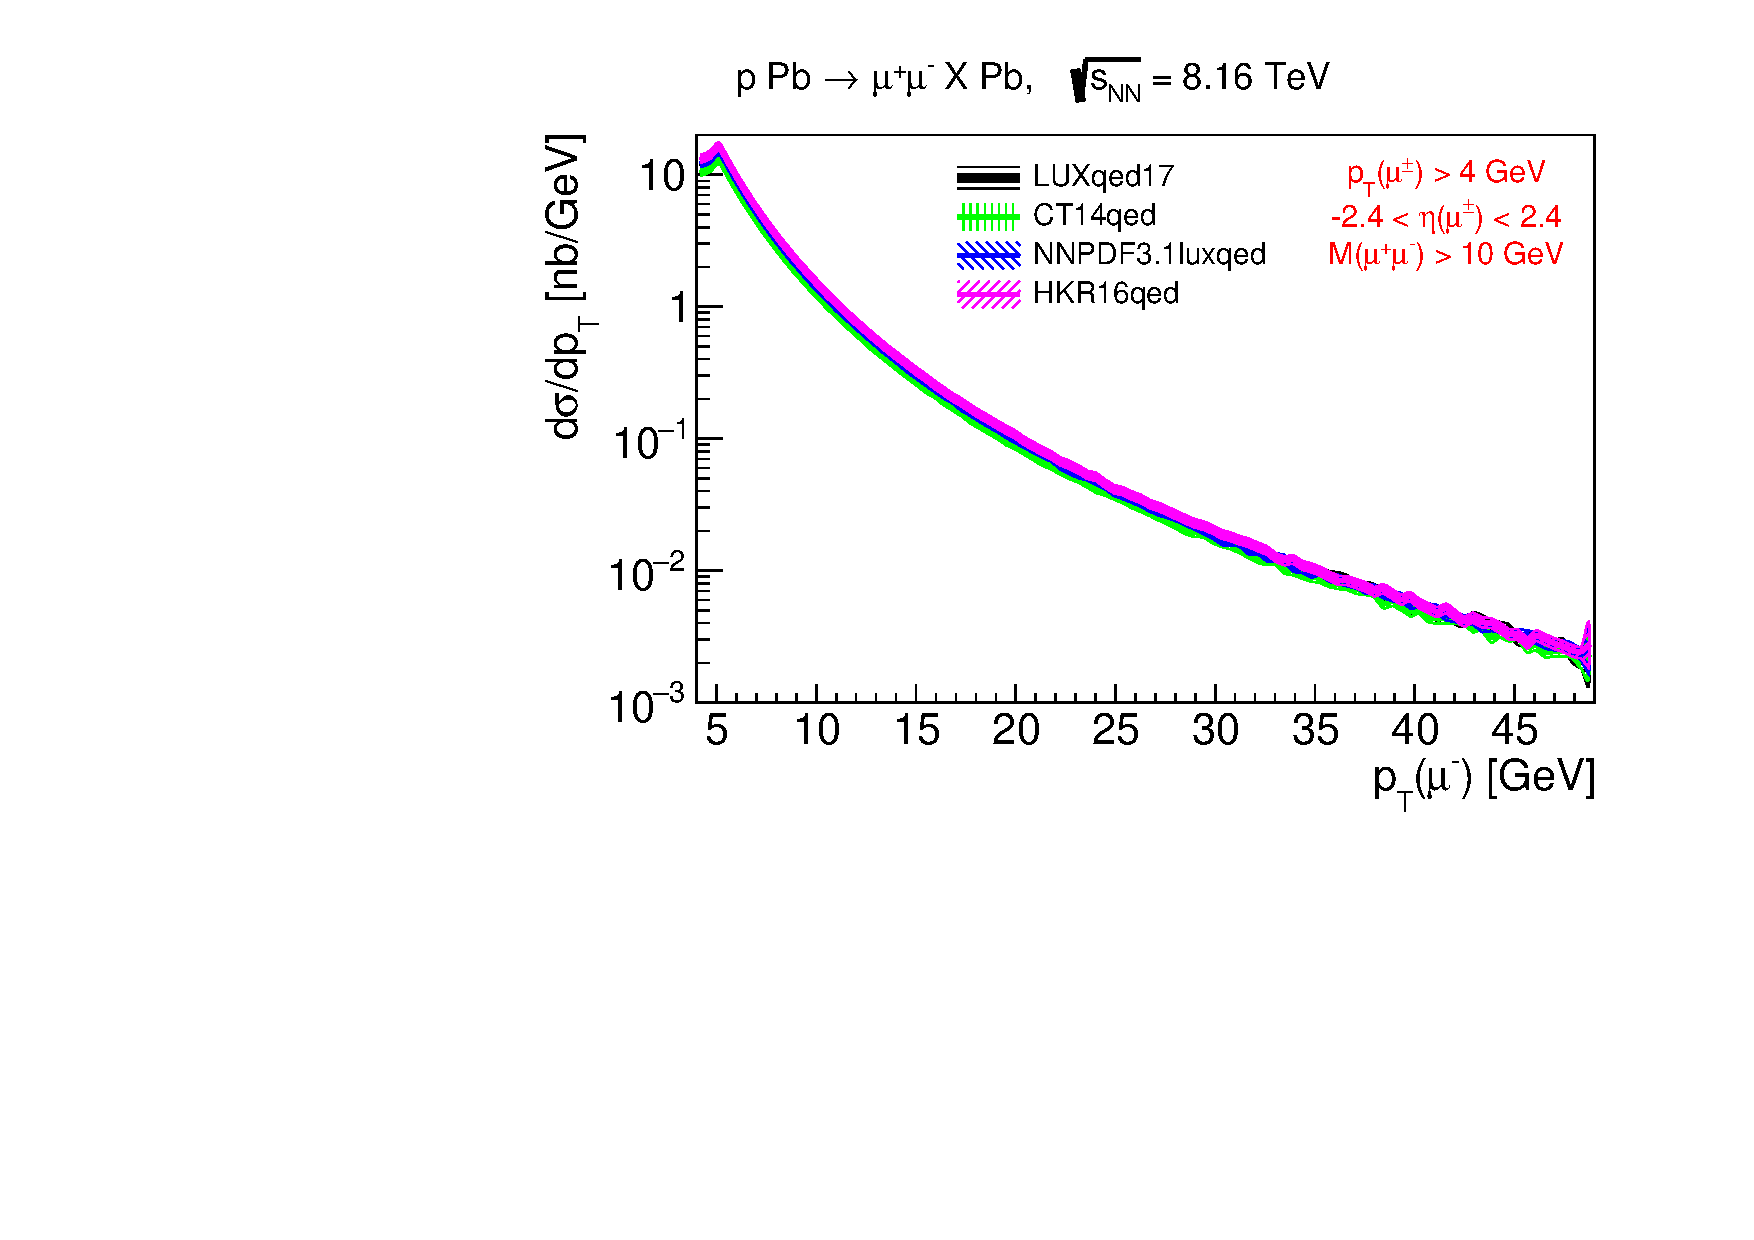
\includegraphics[width=0.43\textwidth]{figures/pTl_inc_cut.pdf}
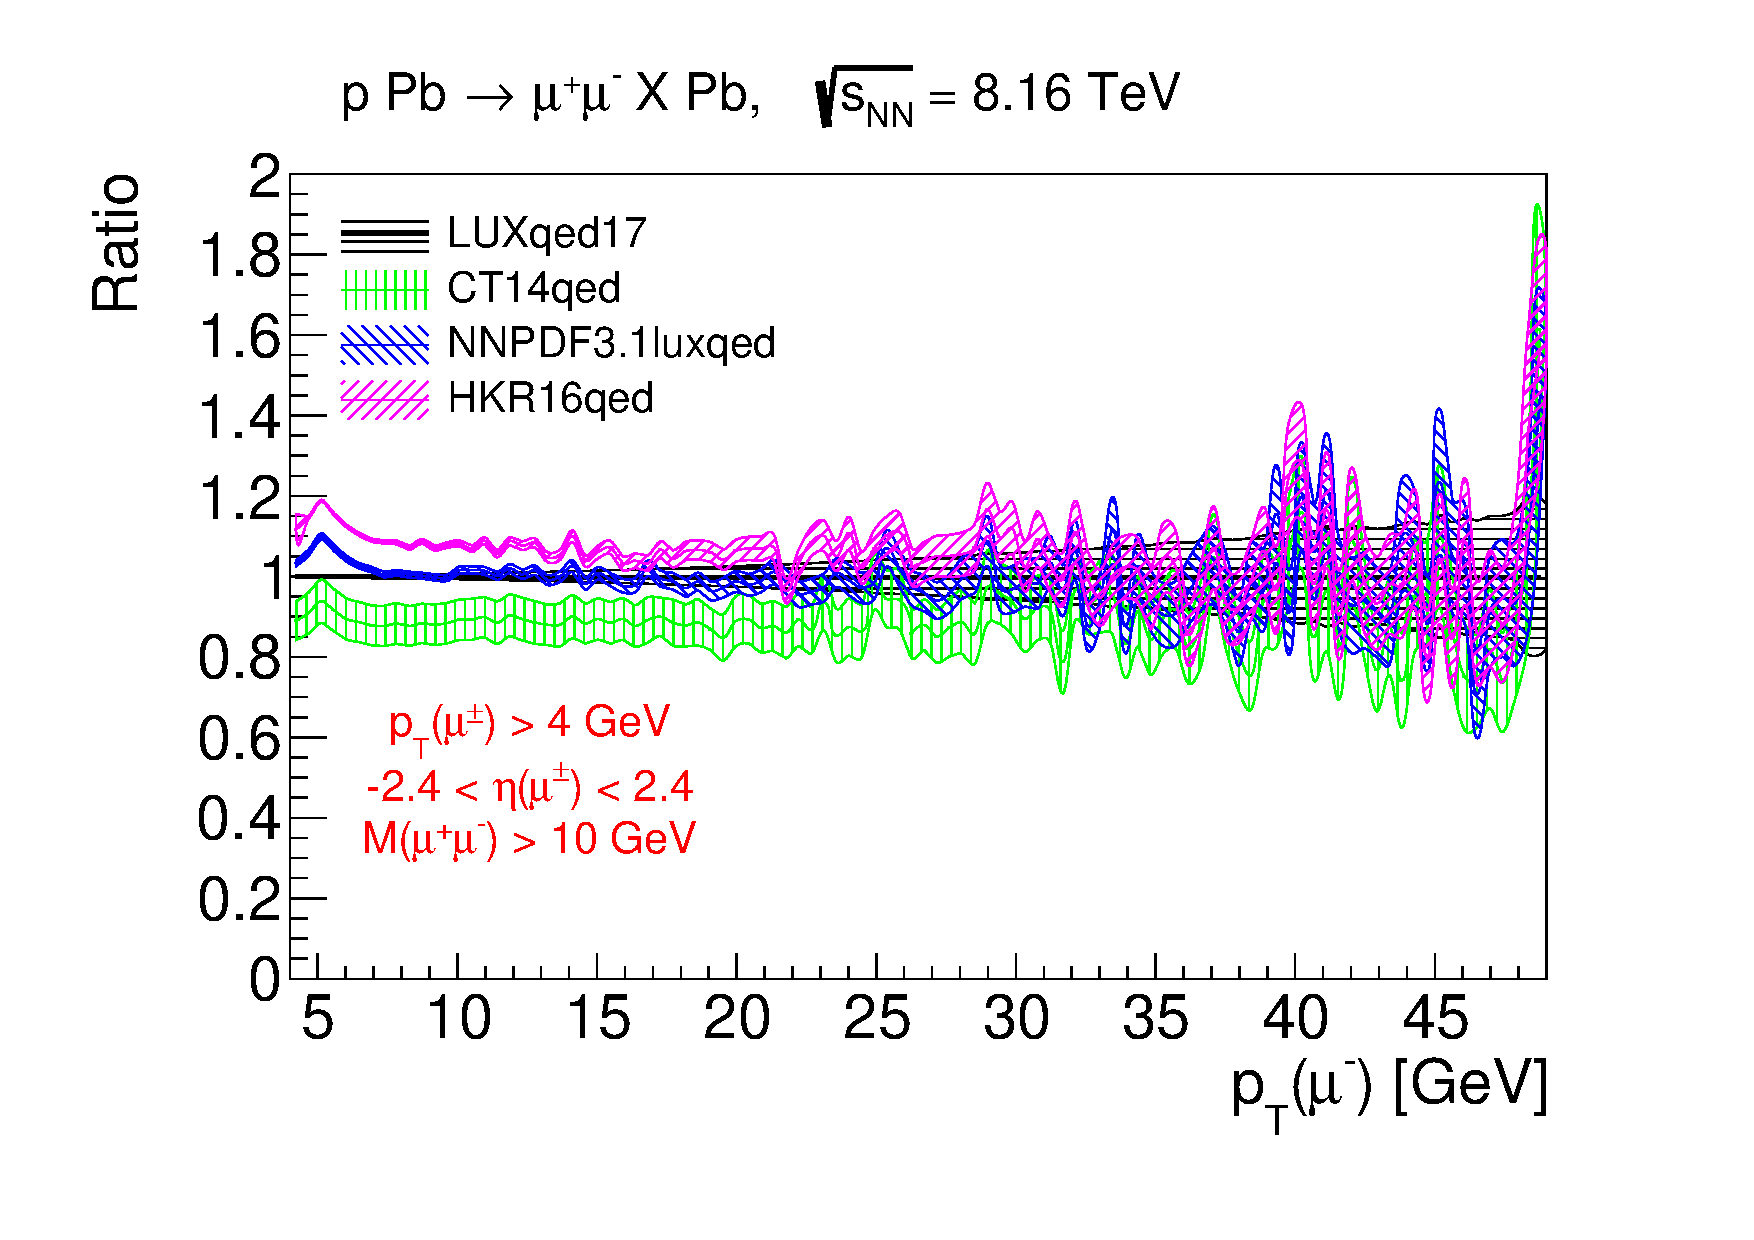
\includegraphics[width=0.43\textwidth]{figures/RatiopTl_inc_cut.pdf}
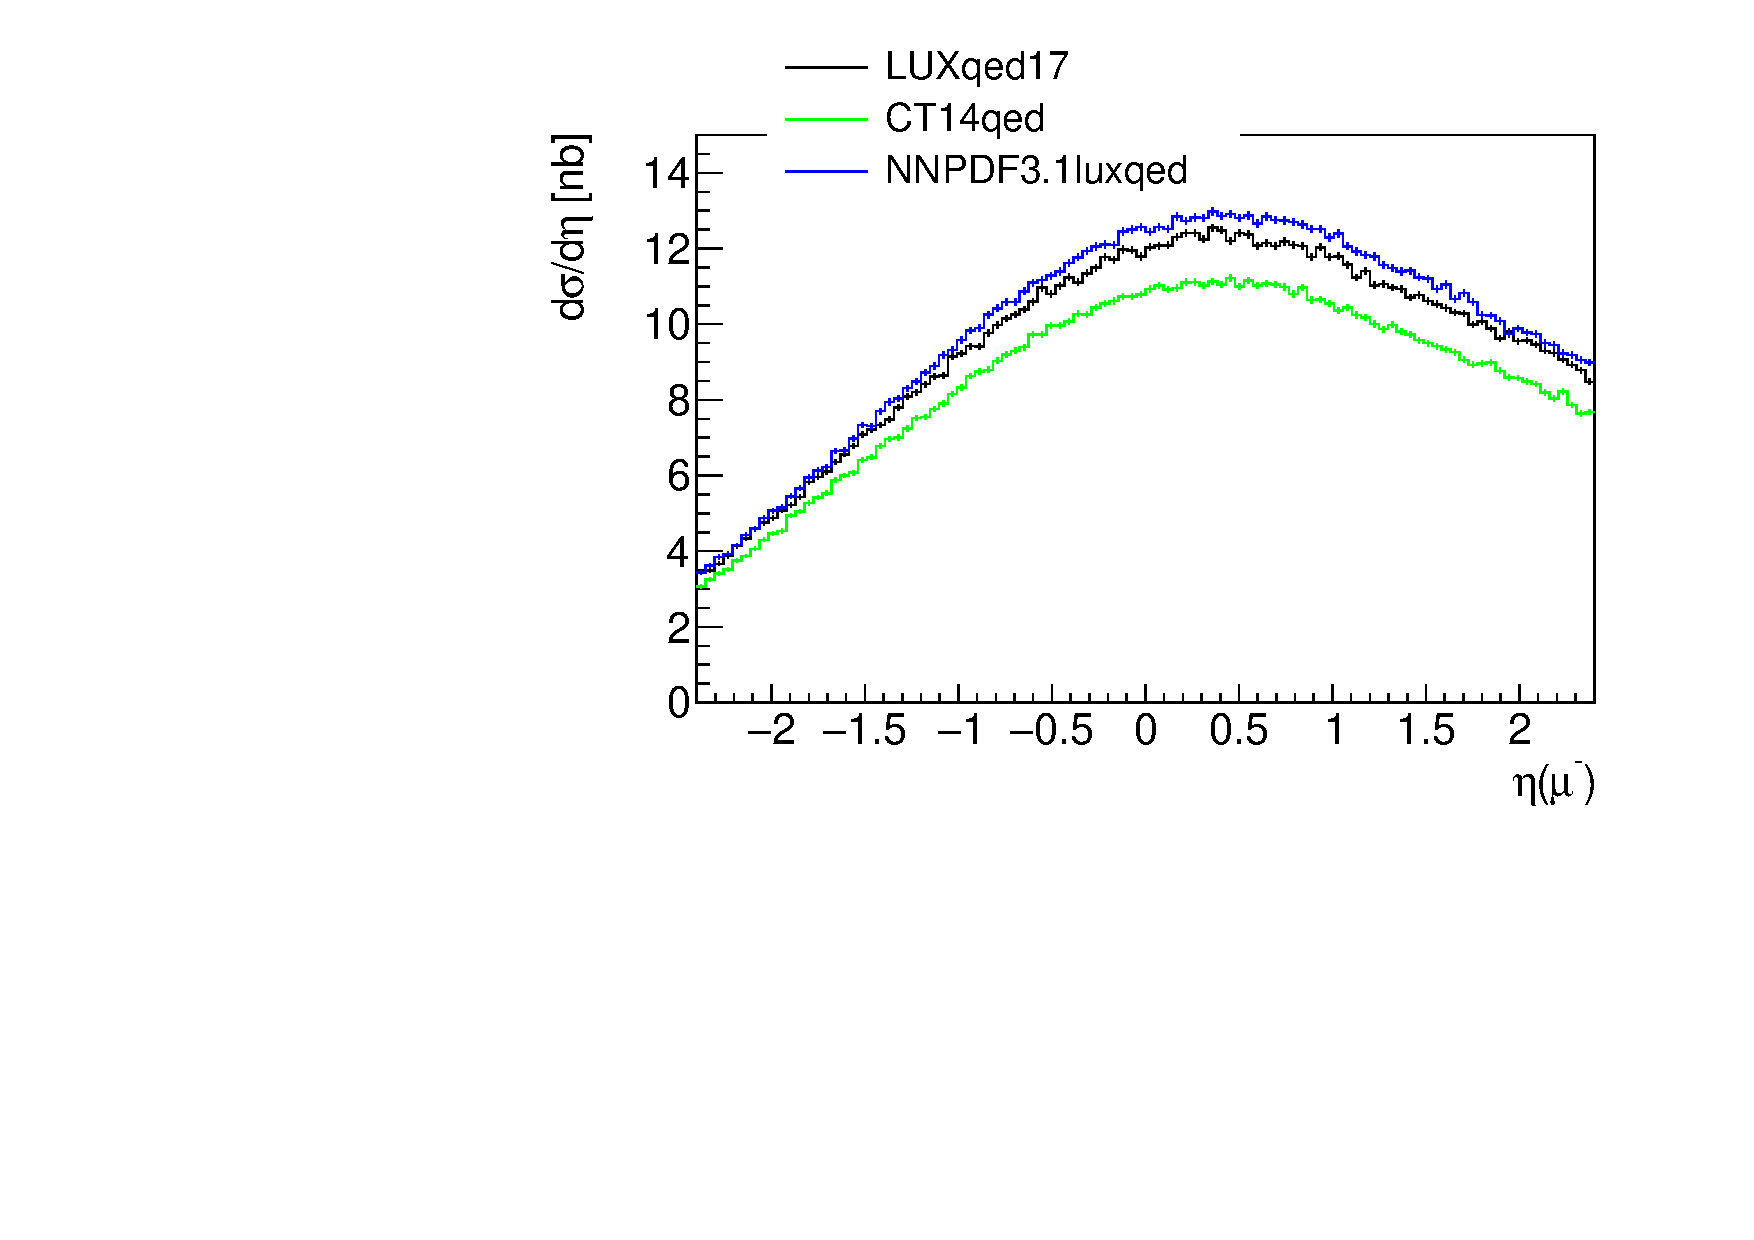
\includegraphics[width=0.43\textwidth]{figures/etal_inc_cut.pdf}
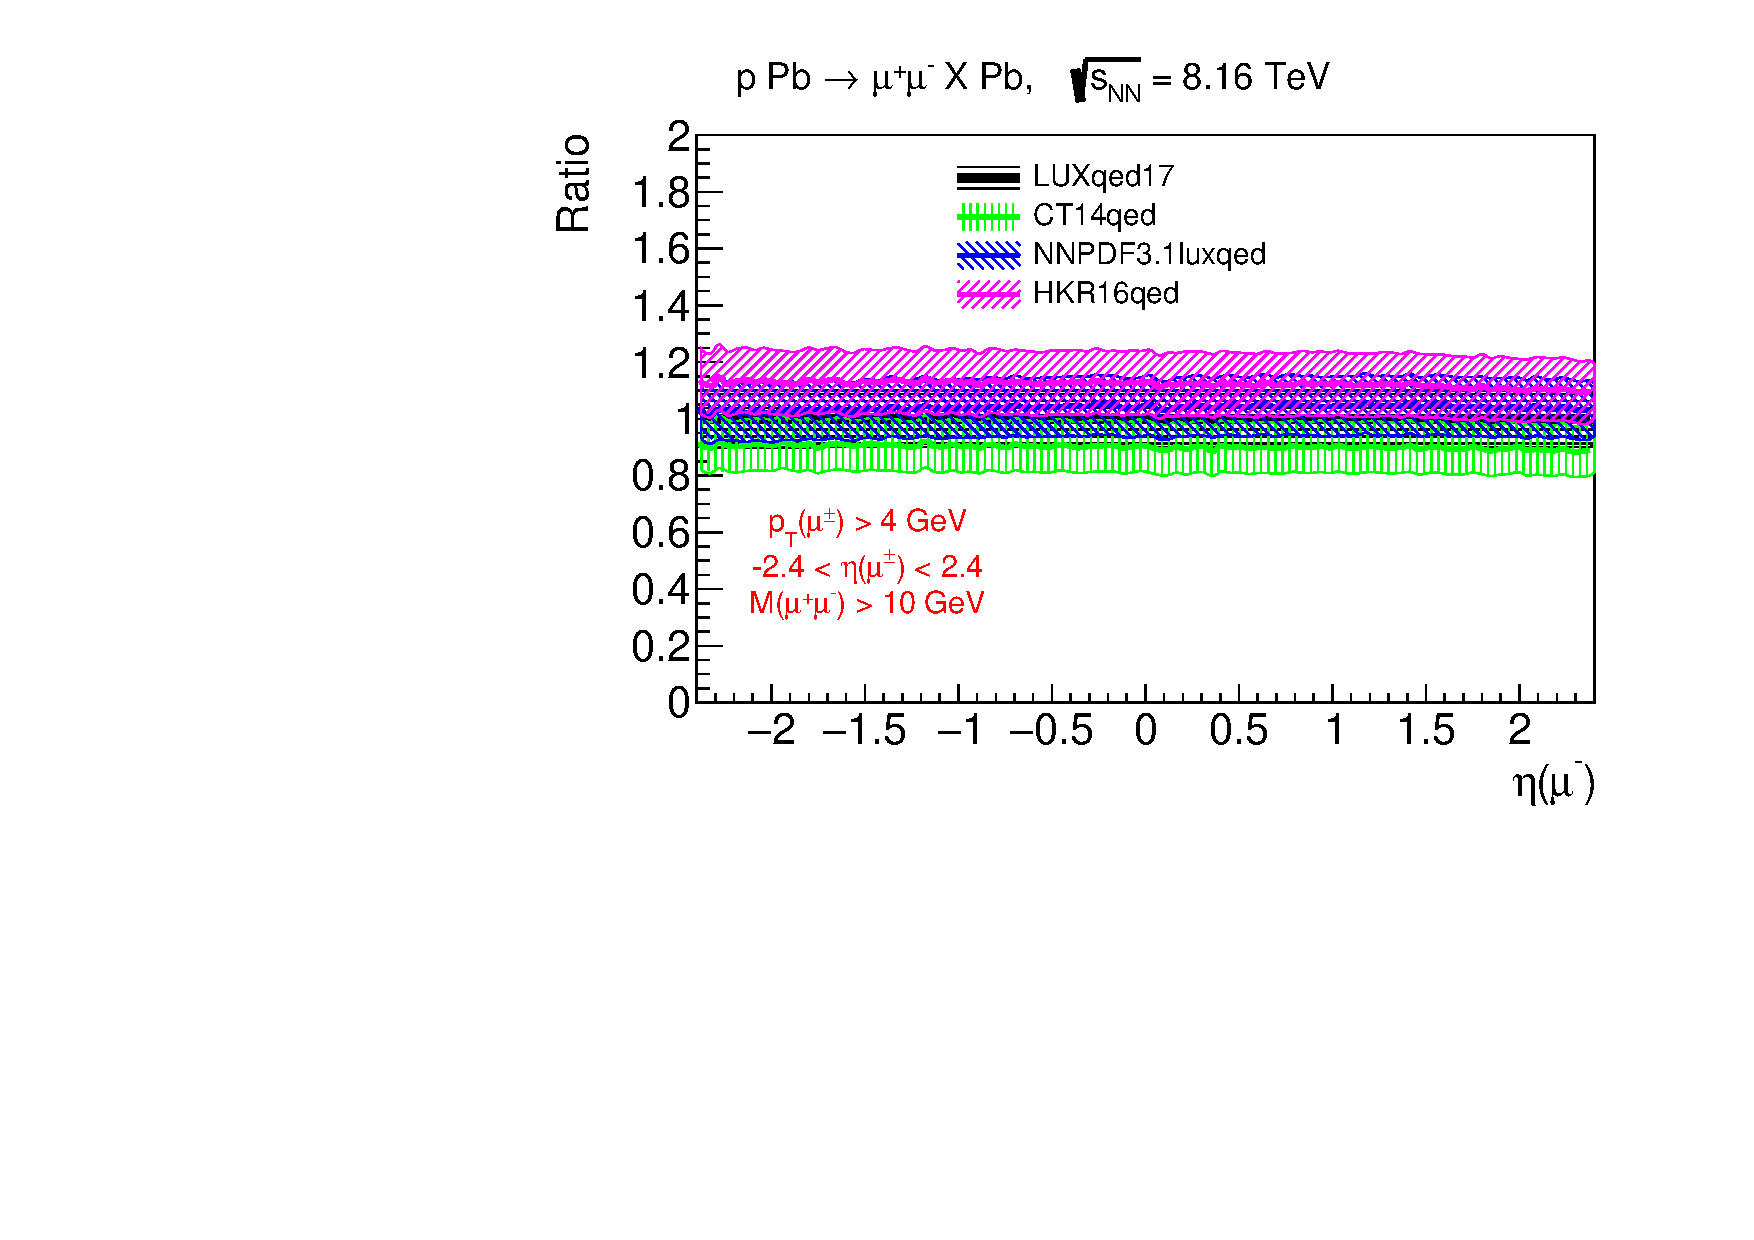
\includegraphics[width=0.43\textwidth]{figures/Ratioetal_inc_cut.pdf}
\caption{Differential cross sections in the fiducial region for $p+\textrm{Pb}\rightarrow \textrm{Pb} + \ell^+\ell^- + X$ production at $\sqrt{s_{N N}} = 8.16$~\TeV\ for different collinear photon PDF sets.
Four differential distributions are shown (from top to bottom): invariant mass of lepton pair, pair rapidity, transverse momentum of negatively-charged lepton and its pseudorapidity. Figures on the right show the ratios to LUXqed17 PDF. The bands denote the PDF uncertainties (if available) calculated at 68\% CL, and the statistical uncertainties of the calculations added in quadrature.}
\label{fig:inc_cut}
\end{figure}

